\documentclass[conference]{IEEEtran}
\IEEEoverridecommandlockouts

% ==========================================
% PACKAGES
% ==========================================
\usepackage{cite}
\usepackage{amsmath,amssymb,amsfonts,amsthm}
\usepackage{algorithmic}
\usepackage{graphicx}
\usepackage{textcomp}
\usepackage{xcolor}
\usepackage{booktabs}
\usepackage{multirow}
\usepackage{url}
\usepackage{float}
\usepackage{hyperref}

% --- TIKZ (Architectural Diagrams) ---
\usepackage{tikz}
\usetikzlibrary{shapes.geometric, arrows, positioning, fit, calc, backgrounds, shadows, trees}

% --- CUSTOM STYLING ---
\setlength{\parskip}{0.5em}
\renewcommand{\baselinestretch}{1.0} 

% --- THEOREM DEFINITIONS ---
\theoremstyle{definition}
\newtheorem{definition}{Definition}
\newtheorem{theorem}{Theorem}
\newtheorem{axiom}{Axiom}
\newtheorem{property}{Property}
\newtheorem{corollary}{Corollary}

\def\BibTeX{{\rm B\kern-.05em{\sc i\kern-.025em b}\kern-.08em
    T\kern-.1667em\lower.7ex\hbox{E}\kern-.125emX}}

\begin{document}

% ==========================================
% TITLE
% ==========================================
\title{The ScholarMaster Architecture: A Unified Reference Model for Privacy-First Intelligent Campus Systems}

% ==========================================
% AUTHOR
% ==========================================
\author{\IEEEauthorblockN{1\textsuperscript{st} Narendra Babu P}
\IEEEauthorblockA{\textit{Dept. of Computer Science} \\
\textit{Swarnandhra College of Eng. \& Tech.}\\
Narsapur, India \\
narendrababu.p@swarnandhra.ac.in}
}

\maketitle

% ==========================================
% ABSTRACT
% ==========================================
\begin{abstract}
Current research in "Smart Campus" technologies suffers from a fragmentation crisis: hardware efficiency, algorithmic accuracy, data privacy, and sociological trust are frequently treated as isolated domains. This paper consolidates the \textbf{ScholarMaster Research Program} into a unified reference architecture that synthesizes 19 component studies into a cohesive doctrine for \textit{Automated Stewardship}. We define the complete vertical stack—from thermal equilibrium in edge silicon to the sociology of student trust—and formalize the \textbf{Canonical Invariant Namespace (INV-01 to INV-15)} that binds these layers together. By defining the operational adversary model ($A_0$--$A_4$) and tracing the end-to-end lifecycle of a spatiotemporal event across the eight-layer boundary, this meta-analysis demonstrates how architectural irreversibility, mandatory governance, and visible privacy converge to solve the "Privacy Paradox" in educational AI. This document serves as the formal architectural reference manual for the entire ScholarMaster Research Program.
\end{abstract}

\begin{IEEEkeywords}
Reference Architecture, System Synthesis, Automated Stewardship, Privacy-by-Design, Smart Campus, Research Roadmap, Threat Modeling.
\end{IEEEkeywords}

% ==========================================
% I. INTRODUCTION: THE FRAGMENTATION CRISIS
% ==========================================
\section{Introduction}
The development of intelligent academic environments is currently stalled by a "Fragmentation Crisis." 



In traditional deployments, system properties are optimized in isolation:
\begin{itemize}
    \item \textbf{Computer Vision} researchers optimize for accuracy (Papers 1, 2) but often ignore the severe thermal constraints and memory bottlenecks of edge deployment (Paper 5).
    \item \textbf{Systems} researchers optimize for high-throughput stream processing (Paper 10) but often neglect the sociotechnical requirements of user trust and consent (Paper 16).
    \item \textbf{Privacy} researchers propose heavy cryptographic protocols (Paper 8) that are computationally infeasible on the constrained hardware required for pervasive deployment (Paper 12).
\end{itemize}

The \textbf{ScholarMaster Architecture} is a direct response to this fragmentation. It is not a single algorithm, but a vertically integrated cyber-physical ecosystem designed to satisfy a complex set of competing constraints: real-time processing latency, strict privacy regulation (GDPR/DPDP), physical hardware endurance, and social legitimacy. 

This paper serves as the \textbf{Unified Reference Model} for the ecosystem. It does not present new experimental data; rather, it synthesizes the findings of the preceding series into a single coherent architectural doctrine. It defines the relationships between the subsystems, establishes the canonical invariants that govern the whole, maps the theoretical proofs to their practical implementations, and establishes the definitive threat model within which the system's privacy claims hold true.

% ==========================================
% II. THE ADVERSARY MODEL
% ==========================================
\section{The Threat Landscape and Adversary Model}
To contextualize the architectural constraints defined in later sections, we must first mathematically define the capabilities of the adversaries the system is designed to thwart. Consolidating the formal definitions from Paper 19, the ScholarMaster architecture operates under a tiered adversary model. 



\subsection{Adversary Classes and Attack Vectors}
\begin{itemize}
    \item \textbf{$A_0$ (Passive Observer):} An entity observing the physical environment or attempting to deduce system state from external hardware behaviors (e.g., LED indicators, thermal signatures). \textit{Defended via:} Transparent signaling paradigms (Paper 15) ensuring the observer has parity with the system's internal state machine.
    \item \textbf{$A_1$ (Network Eavesdropper):} An entity actively sniffing packet traffic on the campus Wi-Fi or LAN, utilizing Man-in-the-Middle (MitM) or replay attacks. \textit{Defended via:} Mutual TLS (mTLS) for all inter-node communication, strictly monotonic nonces to prevent replay, and Differential Privacy (DP) payload noising (Papers 11, 13).
    \item \textbf{$A_2$ (Malicious/Curious Administrator):} An insider with authorized database read access attempting to execute joining attacks or reconstruct historical student behaviors beyond authorized schedules. \textit{Defended via:} Cryptographic hashing of metadata, continuous spatial exclusivity checks, and the absolute L3 irreversibility boundary which destroys raw data before it reaches the persistence layer (Papers 3, 4, 8).
    \item \textbf{$A_3$ (Hardware Thief / Root Access):} A highly capable attacker who physically steals the edge node or utilizes a zero-day exploit to gain OS-level root access. They may attempt cold-boot DRAM freezing or filesystem extraction. \textit{Defended via:} Volatile-Only Processing (`tmpfs`), disabling of swap space, immutable filesystem overlays (OverlayFS), and hardware watchdog timers that force fail-closed halting upon state manipulation (Papers 12, 18).
    \item \textbf{$A_4$ (State-Level Hardware Attacker):} An entity capable of real-time silicon decapsulation, micro-probing NPU buses, or utilizing electron-microscopy to read charge states of deactivated SRAM cells. \textit{This tier is explicitly out of scope for the ScholarMaster architecture.}
\end{itemize}

The architectural invariants presented in this reference model are designed strictly to neutralize adversaries up to and including class $A_3$.

% ==========================================
% III. THE REFERENCE STACK (L1--L8)
% ==========================================
\section{The ScholarMaster Reference Stack}

The architecture is organized into four distinct strata. While Layers 1-8 represent the data flow, the Research Series papers map to these strata to provide operational, logical, and sociological definitions.

% --- FIGURE 1: THE ARCHITECTURE STACK ---
\begin{figure}[htbp]
\centering

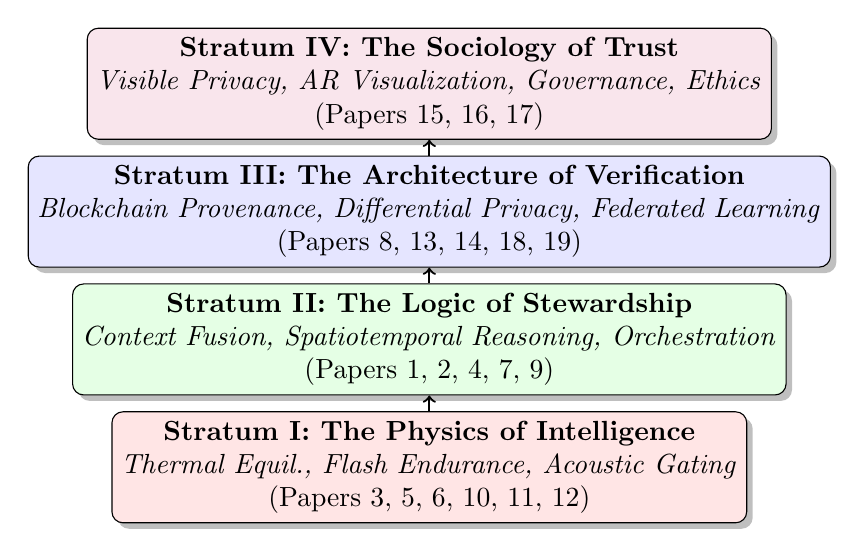
\begin{tikzpicture}[
    node distance=0.2cm,
    layer/.style={rectangle, draw, minimum width=8cm, minimum height=1.2cm, align=center, rounded corners, drop shadow, fill=white},
    label/.style={font=\bfseries\small}
]

% STRATUM 4: SOCIETY
\node[layer, fill=purple!10] (S4) {
    \textbf{Stratum IV: The Sociology of Trust} \\ 
    \textit{Visible Privacy, AR Visualization, Governance, Ethics} \\
    (Papers 15, 16, 17)
};

% STRATUM 3: TRUST
\node[layer, fill=blue!10, below=of S4] (S3) {
    \textbf{Stratum III: The Architecture of Verification} \\ 
    \textit{Blockchain Provenance, Differential Privacy, Federated Learning} \\
    (Papers 8, 13, 14, 18, 19)
};

% STRATUM 2: LOGIC
\node[layer, fill=green!10, below=of S3] (S2) {
    \textbf{Stratum II: The Logic of Stewardship} \\ 
    \textit{Context Fusion, Spatiotemporal Reasoning, Orchestration} \\
    (Papers 1, 2, 4, 7, 9)
};

% STRATUM 1: PHYSICS
\node[layer, fill=red!10, below=of S2] (S1) {
    \textbf{Stratum I: The Physics of Intelligence} \\ 
    \textit{Thermal Equil., Flash Endurance, Acoustic Gating} \\
    (Papers 3, 5, 6, 10, 11, 12)
};

% Connections
\draw[->, thick] (S1) -- (S2);
\draw[->, thick] (S2) -- (S3);
\draw[->, thick] (S3) -- (S4);

\end{tikzpicture}
\caption{The ScholarMaster Unified Reference Stack. The system is built upwards from physical constraints (I) to logical reasoning (II), verified trust (III), and finally social acceptance (IV).}
\label{fig:stack}
\end{figure}

\subsection{Stratum I: The Physics of Intelligence \& Operations}
This layer concerns the physical, thermal, and operational reality of the edge node. It enforces "Privacy by Physics" and operational resilience against harsh deployment conditions.
\begin{itemize}
    \item \textbf{L1 Physical Substrate:} Defined by \textbf{Paper 11} (Production MLOps) and \textbf{Paper 12} (Flash Endurance). This layer establishes the operational runtime, enforcing memory volatility, hardware watchdog supervision, and filesystem immutability via OverlayFS. It bounds the hardware to $A_3$ resistance, ensuring that physical tampering results in immediate cryptographic bricking of the node.
    \item \textbf{L2 Sensor Acquisition:} Validated in \textbf{Paper 5} (Thermal/Memory) and \textbf{Paper 10} (System-Level Validation). Paper 10 provides the empirical survivability validation for the entire L1–L7 stack. Included here is \textbf{Paper 6} (Acoustic Anomaly), handling high-fidelity environmental capture strictly within bounded circular volatile buffers, explicitly preventing paging to physical disk.
\end{itemize}

\subsection{Stratum II: The Logic of Stewardship}
This layer converts raw signals into semantic meaning and governance compliance without reconstructing identity. It bridges the gap between unstructured sensor data and structured logic.
\begin{itemize}
    \item \textbf{L3 Edge Abstraction:} Defined by \textbf{Paper 17} (Irreversibility Doctrine) and \textbf{Paper 3} (Pose Abstraction). This is the absolute "Irreversibility Boundary." High-entropy raw matrices ($D_{raw}$) are destructively compressed into low-dimensional metadata vectors (e.g., 34 geometric keypoints). The original memory blocks containing the raw data are immediately zeroed.
    \item \textbf{L4 Inference:} Validated in \textbf{Paper 1} (Biometric HNSW), \textbf{Paper 2} (Context), and \textbf{Paper 4} (Schedule Compliance). Execution here is identity-blind, context-aware, and strictly bound by the spatiotemporal continuous verification engine (P7). The engine evaluates kinematic constraints to mathematically differentiate valid authorized presence from impossible anomaly states (e.g., topological teleportation).
\end{itemize}

\subsection{Stratum III: The Architecture of Verification}
This layer provides the proofs that the system is behaving as claimed, bridging local logic with global accountability and fault tolerance.
\begin{itemize}
    \item \textbf{L5 Governance:} \textbf{Paper 9} (Orchestration). Enforces policy gates before any data emission. It physically separates the act of algorithmic judgment (L4) from the authorization to transmit, applying time-based and role-based access controls to the metadata stream.
    \item \textbf{L6 Human Output:} \textbf{Paper 15} (AR Visualization) and \textbf{Paper 16} (Sociological Trust). Translates machine boundaries into human-verifiable proof via skeleton-only augmented reality displays, proving to the subjects that the system sees geometry, not identity.
    \item \textbf{L7 Audit Persistence:} \textbf{Paper 8} (Blockchain Provenance). Implements a Byzantine Fault Tolerant (BFT), tamper-evident, append-only local ledger ensuring that $A_2$ adversaries cannot retroactively alter compliance histories or delete evidence of unauthorized system access.
\end{itemize}

\subsection{Stratum IV: The Sociology of Trust}
This layer bridges the gap between isolated edge nodes and the collective institutional intelligence.
\begin{itemize}
    \item \textbf{L8 Federation:} \textbf{Paper 13} (Intra-Campus FL) and \textbf{Paper 14} (Cross-Campus FL). Allows the network to learn global behavioral drifts (e.g., changing illumination patterns over seasons or shifting acoustic baselines) without transmitting local data. It is governed by strict differential privacy (DP) budgets and secure multi-party computation.
\end{itemize}

% ==========================================
% IV. THE CANONICAL INVARIANTS
% ==========================================
\section{The Canonical Invariant Namespace}

To ensure consistency across the 19-paper research program, we formalize the \textbf{ScholarMaster Invariant Namespace}. 



\textit{Note: The invariant namespace does not introduce new enforcement mechanisms but consolidates and labels constraints already validated in component studies (P1, P3, P9, P17, P18).} These invariants act as formal contracts between the system layers; a failure in any invariant triggers an immediate L1 hardware halt.

\subsection{Ephemeral Data Constraints}
\begin{itemize}
    \item \textbf{INV-01 (Raw Non-Persistence):} No sensor data shall persist beyond the L3 boundary (Volatile RAM) \cite{P17, P18}. This guarantees $A_2$ and $A_3$ attackers cannot extract historic imagery.
    \item \textbf{INV-04 (Bounded Temporal Exposure):} Any buffer containing raw data must be explicitly zeroed within a strict temporal window $\Delta_{TTL}$ (e.g., 33ms for 30fps video) \cite{P19}. 
    \item \textbf{INV-09 (Volatile-Only Processing):} All L1-L4 buffers must reside in heap memory mapped to physical RAM. Swap space is disabled at the kernel level, and no disk I/O is permitted for raw data arrays \cite{P12}.
    \item \textbf{INV-10 (Density Constraint):} L3 output dimensionality is strictly capped (e.g., maximum 34 3D keypoints for pose extraction) to ensure mathematical underdetermination, formally preventing the inversion of the neural network back to pixel space \cite{P3}.
\end{itemize}

\subsection{Governance \& Control Flow}
\begin{itemize}
    \item \textbf{INV-02 (Identity Non-Propagation):} Identity tokens are ephemeral, randomly generated per session, and valid only for the immediate execution context; longitudinal tracking across multiple spatial zones via consistent MAC or facial IDs is structurally prohibited \cite{P1, P3, P9}.
    \item \textbf{INV-03 (Governance Non-Bypass):} No data, even abstract metadata, can transition to the network egress module without passing L5 Governance logic checks \cite{P9}.
    \item \textbf{INV-07 (Audit Immutability):} All governance decisions (accept/reject) must be cryptographically hashed and logged to the immutable ledger \textit{before} the corresponding physical or network action is executed \cite{P8}.
    \item \textbf{INV-11 (Consent-Gated Enrollment):} No biometric or behavioral embedding is generated or stored without verified, non-expired, and digitally signed user consent \cite{P8}.
\end{itemize}

\subsection{Distributed Sovereignty}
\begin{itemize}
    \item \textbf{INV-05 (Federation Sovereignty):} No cross-campus model weight update shall contain gradient data allowing the mathematical reconstruction of localized training samples \cite{P14}.
    \item \textbf{INV-12 (Deletion Propagation):} User data deletion/revocation requests must propagate to the global federation state, forcing an unlearning routine within one aggregation round \cite{P14}.
    \item \textbf{INV-13 (Federation Payload Restriction):} L8 egress transmits only DP-noised gradient summaries; explicit data types (images, audio, plaintext logs) are banned at the gRPC schema level \cite{P13}.
\end{itemize}

\subsection{Operational Resilience}
\begin{itemize}
    \item \textbf{INV-06 (Thermal Equilibrium):} Inference load (FPS) must be dynamically throttled to maintain SoC junction temperatures strictly below silicon degradation limits ($T_{junc} < 85^{\circ}C$) \cite{P5, P11}.
    \item \textbf{INV-08 (Fail-Closed Liveness):} System failures (e.g., Watchdog timeouts, TTL expiration, or Out-Of-Memory errors) inevitably transition the node to a HALT/Reboot state, never an OPEN/permissive bypass state \cite{P11}.
    \item \textbf{INV-14 (Non-Disableable Enforcement):} TTL lifecycle checks are hardcoded into the memory allocator's destruction paths and cannot be toggled via runtime configuration files \cite{P18}.
    \item \textbf{INV-15 (Privacy Mode Default):} Following any reboot or power loss, the system inevitably boots into restricted Privacy Mode, requiring an explicit, cryptographically signed remote handshake to elevate privileges \cite{P11}.
\end{itemize}

% ==========================================
% V. INTER-STRATUM COMMUNICATION & LATENCY
% ==========================================
\section{Inter-Stratum Communication and Latency Budgets}
To strictly satisfy INV-04 (Bounded Temporal Exposure limit of 33ms), the architecture requires highly optimized communication protocols between the strata. Traditional microservice architectures relying on HTTP/REST or JSON serialization introduce unacceptable overhead, routinely missing the 33ms window and triggering watchdog halts.

\subsection{Memory Isolation and IPC}
Communication between Stratum I (Acquisition) and Stratum II (Logic) operates entirely via \textbf{Zero-Copy Inter-Process Communication (IPC)}. Raw sensor frames are allocated in contiguous blocks of shared memory (`/dev/shm`). L2 passes only the memory pointer to L3 via lightweight Unix domain sockets. This eliminates the latency of copying multi-megabyte image matrices between processes.

\subsection{The 33ms Pipeline Budget}
The end-to-end latency budget is strictly apportioned:
\begin{enumerate}
    \item \textbf{Sensor Capture \& DMA (L2):} 4ms
    \item \textbf{Neural Network Inference (L3):} 18ms (e.g., executing a quantized MobileNet on the edge NPU).
    \item \textbf{Spatiotemporal Logic \& HNSW (L4):} 6ms. This phase utilizes highly optimized C-structs and cache-aligned Skip Lists (defined in Paper 7) to avoid RAM fetch stalls.
    \item \textbf{Governance \& Ledger Hash (L5/L7):} 3ms.
    \item \textbf{Buffer Destruction (INV-04):} 2ms. Overwriting the original shared memory block with zeros.
\end{enumerate}
If any stage exceeds its allocated budget, the L1 hardware watchdog interrupts the execution thread, zeroes the memory block forcefully, and logs a performance fault to the ledger.

% ==========================================
% VI. THE LIFE OF AN EVENT: END-TO-END TRACE
% ==========================================
\section{The Life of an Event: End-to-End Trace}
To illustrate the interaction of these invariants and the IPC pipeline, consider a student ($S_A$) entering a restricted examination room monitored by a ScholarMaster edge node.



1. \textbf{Ingestion (L1/L2):} Photons hit the camera sensor. A 1080p RGB frame is written via Direct Memory Access (DMA) to a `tmpfs` shared memory buffer. The hardware watchdog starts the strict 33ms countdown (INV-04, INV-09).
2. \textbf{Abstraction (L3):} The IPC pointer is passed to the NPU. A lightweight CNN extracts 34 3D skeletal keypoints (INV-10). \textit{Crucial step:} The original RGB frame in the shared buffer is physically overwritten with zeros (INV-01).
3. \textbf{Reasoning (L4):} The abstract keypoints are evaluated by the Spatiotemporal Logic Engine (Paper 7). The engine checks the previous known location of $S_A$, calculates the kinematic velocity delta, verifies topological adjacency, and queries the local schedule to ensure $S_A$ belongs in this room.
4. \textbf{Governance (L5):} The positive compliance match is packaged into a heavily compressed C-struct tuple. The Governance Filter verifies that active institutional policy permits logging attendance at this specific time and location (INV-03).
5. \textbf{Audit (L7):} The governance decision is hashed using SHA-256 and appended to the local tamper-evident blockchain ledger (INV-07), securing the decision against $A_2$ insider tampering.
6. \textbf{Egress (L8):} Once a day, during off-peak thermal hours, the local model's updated gradient weights (learned purely from abstract keypoint dynamics, not images) are DP-noised and transmitted to the central campus federated aggregator via mTLS (INV-05, INV-13).

At no point in this lifecycle does a human face persist on disk, transmit over a network, or exist in volatile memory beyond the 33ms temporal window.

% ==========================================
% VII. THEOREM-IMPLEMENTATION MAPPING
% ==========================================
\section{The Theorem-Implementation Lattice}
Formal proofs are abstract; engineering is concrete. The formal algebra and theorems are consolidated from P17–P19 and reproduced in Appendix A for reference; no new formal claims are introduced in this document. Table I maps these mathematical theorems to the specific systems engineering implementations validated throughout Papers 1-18.

\begin{table}[htbp]
\caption{Mapping Formal Theorems to System Implementation}
\begin{center}
\begin{tabular}{p{2.5cm} p{2.5cm} p{2.5cm}}
\toprule
\textbf{Formal Theorem (P19)} & \textbf{Enforcement Mechanism} & \textbf{Validation Paper} \\
\midrule
Pixel-Space Non-Reconstructability & Pose-Only Abstraction & Paper 3 (Pose) \\
& Spectral Gating & Paper 6 (Audio) \\
\midrule
Bounded Exposure Window ($\Delta \le 33$ms) & TTL Enforcement Loop & Paper 18 (Runtime) \\
& \texttt{mlock} / OverlayFS & Paper 12 (Flash) \\
\midrule
Governance Non-Bypass & Policy Gate Logic & Paper 9 (Orch.) \\
& Cryptographic Token & Paper 8 (Ledger) \\
\midrule
Fail-Closed Reachability & Watchdog Process & Paper 18 (Runtime) \\
& Systemd Supervision & Paper 11 (Ops) \\
\midrule
Approximate Retrieval Isolation & HNSW Indexing & Paper 1 (Biometric) \\
& Fixed-Time Graph & Paper 19 (TCB) \\
\bottomrule
\end{tabular}
\end{center}
\end{table}

% ==========================================
% VIII. CONCLUSION
% ==========================================
\section{Conclusion: From Papers to Program}
The ScholarMaster project began with a specific engineering question: \textit{Can we measure student engagement automatically?} Over the course of this 19-paper research arc, the question evolved into something far more fundamental: \textit{Can we build intelligent systems that are inherently trustworthy?}

This unified reference model demonstrates that the answer is yes, but only if we systematically abandon the "patchwork" approach to AI systems. Trust cannot be appended later via legal compliance documents or arbitrary cloud access controls; it must be structurally compiled into the runtime constraints of the edge silicon. By vertically integrating physical hardware constraints (L1), formal kinematic logic (L4), and sociological visibility design (L6), the ScholarMaster Architecture provides a reproducible, mathematically grounded blueprint for the next generation of privacy-preserving civic AI.

% ==========================================
% APPENDICES
% ==========================================
\appendices

\section{Unified Formal Appendix}
\label{sec:appendix_theorems}

This appendix consolidates the formal definitions and theorems established throughout the ScholarMaster Research Series.

\textit{Threat Model Scope Clause:} All formal guarantees presented herein are bounded by the adversary classes $A_0$ (Passive Observer) through $A_3$ (Root Access/Physical Theft) as defined in Section II. Defense against $A_4$ (State-Level Silicon Decapsulation) is strictly outside the scope of this architecture.

% ==========================================
\subsection{Privacy \& Architectural Irreversibility}

\begin{definition}[Architectural Irreversibility \cite{P3, P17}]
Raw biometric data $D_{raw}$ cannot propagate beyond a designated \textit{Volatile Zone} $Z_V$ to the \textit{Persistent Zone} $Z_P$ by architectural constraint.
\begin{equation}
\forall t, \quad D_{raw}(t) \in Z_V \implies D_{raw}(t) \notin Z_P
\end{equation}
\end{definition}

\begin{theorem}[Pixel-Space Non-Reconstructability \cite{P19}]
Let $f: \mathbb{R}^{H \times W} \to \mathbb{R}^{d_{meta}}$ be the feature extraction function executed at L3. The exact reconstruction of the raw biometric matrix $X$ from post-boundary representation $Y$ is architecturally precluded provided:
\begin{equation}
\text{rank}(f) \le d_{meta} \ll H \times W
\end{equation}
Consequently, $\text{Ker}(f) \neq \{0\}$, implying $f$ is massively non-injective and the inverse problem is mathematically ill-posed without massive external auxiliary data.
\end{theorem}

\begin{corollary}[Information Loss]
Because the mapping $f$ intentionally discards texture, lighting, and background components to isolate pure geometric coordinates (e.g., 34 skeletal keypoints), the conditional entropy $H(X|Y)$ approaches $H(X)$, rendering statistical recovery techniques computationally intractable under adversary models up to $A_3$.
\end{corollary}

\begin{property}[Bounded Temporal Exposure \cite{P19}]
The system enforces that any memory buffer $b$ containing raw data must be explicitly zeroed within the strict configured temporal window $\Delta_{TTL}$.
\begin{equation}
\square \left( (Alloc(b) \land Raw(b)) \implies \Diamond_{\le \Delta_{TTL}} Zeroed(b) \right)
\end{equation}
\end{property}

\begin{theorem}[Identity Non-Propagation \cite{P9}]
Identity reconstruction in higher layers is precluded under the defined adversary model ($A_0$--$A_3$), assuming no auxiliary side-channel data and provided the spatial zone $\zeta$ enforces k-anonymity over the aggregation window $\Delta t$:
\begin{equation}
\forall e \in \zeta, \quad |\text{Subjects}(\zeta, \Delta t)| \ge k
\end{equation}
where $k \ge 2$, ensuring no single trajectory can be isolated from the aggregate data flow.
\end{theorem}

% ==========================================
\subsection{System Stability \& Trust Boundaries}

\begin{definition}[Trusted Computing Base (TCB) \cite{P19}]
The set of components critical to privacy invariants is strictly defined as:
\begin{equation}
TCB = \{ C_{boot}, C_{kernel}, C_{alloc}, C_{sched}, C_{gov} \}
\end{equation}
The TCB explicitly \textbf{excludes} AI inference models, User Interfaces, the MQTT messaging broker, and the Blockchain layer ($\mathcal{U}$). By isolating the TCB from the complex, non-deterministic AI runtimes, the system guarantees that a compromise in the neural network weights (e.g., an adversarial perturbation attack) cannot bypass the structural governance controls.
\end{definition}

\begin{property}[Governance Gate Non-Bypass \cite{P9}]
No data can transition to network egress ($Net$) without passing L5 Governance checks ($Gov$).
\begin{equation}
\square \left( Emit(b) \implies Gov(b) \right)
\end{equation}
\end{property}

% ==========================================
% REFERENCES (THE FULL CORPUS)
% ==========================================
\begin{thebibliography}{00}

\bibitem{P1} N. Babu P., "Scalable High-Throughput Biometric Identification using HNSW," \textit{ScholarMaster Series}, 2025.
\bibitem{P2} N. Babu P., "Context-Aware Multi-Modal Framework," \textit{ScholarMaster Series}, 2025.
\bibitem{P3} N. Babu P., "Privacy-Preserving Academic Engagement Metrics," \textit{ScholarMaster Series}, 2025.
\bibitem{P4} N. Babu P., "Automated Schedule-Compliance Monitoring," \textit{ScholarMaster Series}, 2025.
\bibitem{P5} N. Babu P., "Benchmarking Unified Memory Architectures," \textit{ScholarMaster Series}, 2025.
\bibitem{P6} N. Babu P., "Privacy-Preserving Acoustic Anomaly Detection," \textit{ScholarMaster Series}, 2025.
\bibitem{P7} N. Babu P., "Spatiotemporal Rule-Based Reasoning," \textit{ScholarMaster Series}, 2025.
\bibitem{P8} N. Babu P., "Trust-Aware Metadata Provenance," \textit{ScholarMaster Series}, 2025.
\bibitem{P9} N. Babu P., "Privacy-Governed Multi-Module Orchestration," \textit{ScholarMaster Series}, 2025.
\bibitem{P10} N. Babu P., "System-Level Validation of Smart Campus Intelligence," \textit{ScholarMaster Series}, 2025.
\bibitem{P11} N. Babu P., "Production-Grade Edge MLOps Architecture," \textit{ScholarMaster Series}, 2026.
\bibitem{P12} N. Babu P., "Flash Endurance Engineering for Edge AI," \textit{ScholarMaster Series}, 2026.
\bibitem{P13} N. Babu P., "Intra-Campus Federated Learning," \textit{ScholarMaster Series}, 2026.
\bibitem{P14} N. Babu P., "Cross-Campus Federated Intelligence," \textit{ScholarMaster Series}, 2026.
\bibitem{P15} N. Babu P., "Augmented Situation Awareness (AR)," \textit{ScholarMaster Series}, 2026.
\bibitem{P16} N. Babu P., "Beyond the Panopticon: Sociological Trust," \textit{ScholarMaster Series}, 2026.
\bibitem{P17} N. Babu P., "Architectural Irreversibility (Capstone)," \textit{ScholarMaster Series}, 2026.
\bibitem{P18} N. Babu P., "Runtime Enforcement of Irreversibility," \textit{ScholarMaster Series}, 2026.
\bibitem{P19} N. Babu P., "Formal Threat Model and TCB Definition," \textit{ScholarMaster Series}, 2026.

\end{thebibliography}

\end{document}
